\chapter{\LaTeX 與 packages 的使用}
\href{https://en.wikibooks.org/wiki/LaTeX}{wikibook} 
的 {\LaTeX} 講解與分類很好,且都是標準 package ,剩下的都是屬於更
細微的調整,所以最後只是去找 package 的詳細 reference 說明使用而已。
\\\\
{\LaTeX} 如果是多檔使用,可以用
\begin{verbatim}
\begin{docuemnt}
\include{chapter1}
 或者
\input{chapter1.tex}
\end{document}
\end{verbatim}
include 一定要是 .tex 副檔名,且不可寫副檔名,
input 則可以使用別的副檔名,副檔名可寫可不寫。

\section{書籍排版元素}
除了基本的章節段落 \verb=\chapter{} \section{} \subsection{} \paragraph{}=,
強迫分行使用兩個反斜線,\verb=\\=,所以空一行就要 \verb=\\\\=
,或者用 \verb=\\[1cm]= 指定換行空白大小。光這樣其實就可以編幾頁文章了。
\\\\
最重要的單位元素其實是 paragraph (par),很多排版的規矩,縮排,對齊,大小,
留白, 都是以 paragraph 為根本,它會在版面上形成一個小盒子,盒子內的文字
太多才會自動折行, 在後面像圖表等使用,後面都是這小盒子。 
\\\\
幾個常用基本書籍文章邏輯元素使用,例如
\begin{itemize}
\item 封面 title page
\item 目錄 table of content TOC 每本書的目錄。
\item 註腳 footnote 在書頁底下特別說明本頁中特定詞彙。
\item 列舉 list 不同的列舉。
\item 參照 cross reference 整本
\item 索引 index 在書後面讓人好找到特別詞彙。
\item 參考文獻 bibliography
\end{itemize}

\subsection{Title and TOC}
title 與 TOC 範例,主要是那個 maketitle 與 tableofcontents 要在 document 裡面。
如果只有一位作者,那就不需要那個 and 了。
\begin{verbatim}
\documentclass[a4paper,10pt]{book}

\title{Linux Kernel Driver}
\author{
  Alibuda Huang \\
  alibuda\_huang@yahoo.com \\
  \and 
  Asaburu Liu \\
  asaburu\_liu@gmail.com \\
  Gyoza Publisher
}

\begin{document}
\maketitle
\tableofcontents
...
\end{document}
\end{verbatim}
TOC 要注意的就是要跑兩次引擎,第一次產生 .toc 檔,第二次才會真正在裡面產生
漂亮的 TOC。
\subsection{footnote}
footnote 範例
\begin{verbatim}
宅男\footnote{一種胖胖的可愛動物}
\end{verbatim}
宅男\footnote{一種胖胖的可愛動物}
\subsection{list}
list 是最常用到元素,有三種
\begin{verbatim}
\begin{itemize}
\item 最簡單前面圓點 list 1
\item 最簡單前面圓點 list 2
  \begin{enumerate}
  \item 不用寫1
  \item 不用寫2
    \begin{description}
    \item [item1] item1 會變粗體
    \item [item2] item2 會變粗體
    \end{description}
  \end{enumerate}
\item 最簡單前面圓點 list 3
\end{itemize}
\end{verbatim}
\subsection{cross reference}
corss reference\label{sec:ref} 用在參考圖表或某段特定文字
\begin{verbatim}
在某處設下 mark 這個 label
\label{sec:mark}
....
在別的地方用 \ref 與 \pageref
.....
請參照 第\ref{sec:mark} 節
在第 \pageref{sec:mark} 頁中
\end{verbatim}
有 ref (\ref{sec:ref}) 的也要跑兩次引擎才有用。
其中大家現在有個不成文規矩是 cross reference 內的 label 中,key 用
\begin{itemize}
  \item sec:xxx 表示 section, page
  \item fig:xxx 表示圖形
  \item tab:xxx 表示 table
  \item equ:xxx 表示數學式子
\end{itemize}
表示不同的 cross reference id key。
\subsection{index}
index 索引製作必須要有 makeidx package,makeindex 命令必須放在 preamble ,
然後 文章裡面用 index 命令加到索引資料庫 ,最後 printindex 印出
\begin{verbatim}
\usepackage{makeidx}
\makeindex
.....
文字\index{索引key@文字印出格式}
....

\printindex
....
\end{verbatim}
這個 index\index{index@index} 裡面的長相可以由後面的格式設定決定,還瞞複雜沒規則的
\begin{center}
\begin{tabular}{ccp{4cm}}
命令 & 意義 \\
\hline
\verb=哈囉\index{hello}= &  用 hello \index{hello} 做索引 key 並印出 hello 頁數\\
\verb=hello\index{hello@哈囉}=& 在索引頁會印出哈囉\index{hello@哈囉}\\
\verb=\index{hello!world}= & 會在 hello 下面印出空格斜體的 world \index{hello!world} 表示是 sub index\\
\verb=\index{hello|emph}= & 頁數用 emph 方法印出 \index{hello|emph} \\
\verb=\index{hello@\emph{hello}}=& hello 用emph印出\index{hello@\emph{hello}}\\
\end{tabular}
\end{center}
\printindex
它這跟TOC, reference 一樣,要跑兩次,而且要額外用 makeindex 程式處理之前產生的 idx 檔
\begin{verbatim}
$ xelatex latex.tex; makeindex latex.idx; xelatex latex.tex
\end{verbatim}
\subsection{bibliography}
bibliography 用在論文或書後面,使用thebibliography 環境與 cite 命令來引用,
跟之前 lable 或 index 一樣有 key 值參照。以下範例,99 只是印出文獻時,前面
數字編號的字體寬度,不知道為什麼當初是這樣設計的參數。
\begin{verbatim}
\cite{kernel}


.....
\begin{thebibliography}{99}
  \bibitem{kernel}Linux Kernel Development Third Edition
        Addison Wesley, ISBN-13: 978-0-672-32946-3
  \bibitem{ldd3}Linux Device Drivers, 3rd Edition
        O'Reilly , ISBN-13: 978-0596005900
  \bibitem[docs]{docskernel} http://docs.kernel.org
  \bibitem[os]{osdev} http://wiki.osdev.org
  \bibitem{gitkernel}
        https://linux-kernel-labs.github.io/refs/heads/master/
\end{thebibliography}
\end{verbatim}
\begin{tabular}{cc}
命令 & 效果 \\
\hline
\verb=\cite{kernel}=& \cite{kernel} \\
\verb=\cite{docskernel}=& \cite{docskernel}\\
\verb=\cite[alibuda,LDD3]{osdev,ldd3}=& \cite[alibuda,LDD3]{osdev,ldd3}\\
\verb=\cite[docs.kernel.org]{docskernel}=& \cite[docs.kernel.org]{docskernel}\\
\verb=\cite{osdev}=& \cite{osdev}\\
\end{tabular}
\begin{thebibliography}{99}
  \bibitem{kernel}Linux Kernel Development Third Edition
        Addison Wesley, ISBN-13: 978-0-672-32946-3
  \bibitem{ldd3}Linux Device Drivers, 3rd Edition
        O'Reilly , ISBN-13: 978-0596005900
  \bibitem[docs]{docskernel} http://docs.kernel.org
  \bibitem[os]{osdev} http://wiki.osdev.org
  \bibitem{gitkernel}
        https://linux-kernel-labs.github.io/refs/heads/master/
\end{thebibliography}

\section{字形設定}
字型是讓整個文章排版成功的最重要設定,但原本的引擎plain \TeX 或 pdftex 
有很多限制
\begin{itemize}
\item 內定用 Computer Modern 字型,metafont 格式,OT1 編碼向量字,
很多設定family, 斜體,大小等等其實都只是在設定 CM font 而已。並沒有很好統一
的方法選取不同字型。
\item 原本引擎使用 NFSS, 要有 font metric 檔還有相關map, fd 定義檔建造好才能
使用新字型, 這些資訊檔,一般要靠工具擷取出來,是 distro 幫我們建造好的,因
此沒有建造就無法使用新字型。除非對整個 \TeX 很熟的人,不然新手是叫苦連天。
\end{itemize}
在新的xetex, luatex 可以使用 \href{https://texdoc.org/index.html}{fontspec}
這個 macro 來 run time 時邊擷取出
font metric 等資訊,邊做排版,所以用 CJK 相關套件時,其實後面都是用上 fontspec
這個套件。即使創造新命令也是相近的 macro 名稱。
\begin{verbatim}
\usepackage{fontspec}
\setmainfont{Georgia}
\setsansfont{Arial}
\setmonofont{Arial}

\begin{document}
alibuda
\end{verbatim}
setmainfont, setsansfont, setmonofont 後面的參數可以直接是檔名,也可以是
fc-list 抓出來藏在字型檔裡面的字型名,fc-list 抓出的第一與第二欄位都可以。
而如果跟中文的 setCJKmainfont 一起用,則可以中文英文分開來。
\\\\
選定字型後才是字型參數變換,
就是那些斜體,大小等等設定,這些是原本 \LaTeX 就有的 macro 設定。
\\\\

家族,粗斜體設定

\begin{description}
  \item [Family] - \verb=\textrm{} \textsf{} \texttt{}=
  \item [Weight] - \verb=\textbf{} - bold, \textmd{} - medium=
  \item [Shape] - \verb=\textup{}, \textit{}, \textsl{}=
\end{description}

大小設定

\begin{center}
\begin{tabular}[t]{lll}
命令 & 效果 & 在本文是10pt的相對大小 \\
\hline
\hline
\verb=\tiny{tiny}= & \tiny{tiny} & 5pt \\
\verb=\scriptsize{scriptsize}= & \scriptsize{scriptsize} & 7pt \\
\verb=\footnotesize{footnotesize}= & \footnotesize{footnotesize} & 8pt \\
\verb=\small{small}= & \small{small} & 9pt \\
\verb=\normalsize{normalsize}= & \normalsize{normalsize} & 10pt \\
\verb=\large{large}= & \large{large} & 12pt \\
\verb=\Large{Large}= & \Large{Large} & 14.4pt \\
\verb=\LARGE{LARGE}= & \LARGE{LARGE} & 17.28pt \\
\verb=\huge{huge}= & \huge{huge} & 20.74pt \\
\verb=\Huge{Huge}= & \Huge{Huge} & 24.88pt \\
\end{tabular}
\end{center}
上面都是一些已經定義好方便用的,也就是排版這麼多年有些約定成俗的規格,
大小設定命令格式是三種都有,所以它也有 environment begin, end 使用。
而直接選擇大小
\begin{verbatim}
\fontsize{5cm}{5.5cm}\selectfont
\end{verbatim}
5.5cm 是 line space 行距。前面 5cm 不寫單位就是用 pt,一個 pt 在
不同地方大小不太一樣,但大概是 0.35mm
\begin{itemize}
\item American standard : 0.35136 mm. 
\item Computer standard : 0.3527 mm 
\item European standard : 0.37597151 mm
\end{itemize}

最後其他一些效果

\begin{center}
\begin{tabular}[t]{lll}
命令 & 效果 & 作用 \\
\hline
\hline
\verb=\emph{emph}= & \emph{emph} & 強調 \\
\verb=\underline{underline}= & \underline{underline} & 底線  \\
\verb=\uppercase{uppercase}= & \uppercase{uppercase} & 大寫  \\
\verb=\lowercase{LOWERCASE}= & \lowercase{LOWERCASE} & 小寫  \\
\end{tabular}
\end{center}

%\begin{uppercase}
%alibuda is a asaburu
%\end{uppercase}
更複雜的都要自己寫 macro 了。

\section{一些設定範本}
\LaTeX 有內定標準 package ,但有的不是很常用,
一些簡單 package 的設定能讓呆板醜醜的內定設定變得漂亮。
\begin{itemize}
\item \href{https://ctan.math.utah.edu/ctan/tex-archive/macros/latex/contrib/xcolor/xcolor.pdf}{xcolor}
能夠上顏色的 package。
\item \href{https://ctan.math.illinois.edu/macros/latex/contrib/hyperref/doc/hyperref-doc.pdf}{hyperref}
能夠做像 html 跳來跳去連結 link 的功能。
\item \href{http://tug.ctan.org/tex-archive/macros/latex/contrib/fancyhdr/fancyhdr.pdf}{fancyhdr}
能夠做頁眉上的提示。
\item \href{https://ctan.math.utah.edu/ctan/tex-archive/macros/latex/contrib/listings/listings.pdf}{listings}
能夠用來寫程式語言的表現。
\end{itemize}

\subsection{xcolor}
設定顏色的 package ,很多其他 package 都以這個為基底加上顏色功能。
為了使用一些好記的顏色名字,多加 dvipsnames 在
\verb=\usepackage[dvipsnames]{xcolor}=
而且有的名字是大小寫有差別的。
\begin{center}
\begin{tabular}{ccc}
命令 & 效果 \\
\hline\hline
\verb=\color{blue}{blue}= & \color{blue}{blue} & \\
\verb=\textcolor{NavyBlue}{NavyBlue}= & \textcolor{NavyBlue}{NavyBlue} & \\
\verb=\colorbox{green}{green background}= & \colorbox{green}{green background} & \\
\verb=\fcolorbox{green}{yellow}{green frame}= & \fcolorbox{green}{yellow}{green frame} & \\
\verb=\color[cmyk]{0,1,0,0}{red}= & \color[cmyk]{0,1,0,0}{red} \\
\verb=\definecolor{myred}{rgb}{1,0,0}\color{myred}{myred} = &
 \definecolor{myred}{rgb}{1,0,0}\color{myred}{myred} \\
\end{tabular}
\end{center}

\subsection{hyperref}
這會讓 hyperlink 字包括目錄 TOC 是藍色的。在\verb=\begin{document}=前先設定
\begin{verbatim}
\hypersetup{
  backref,
  unicode=true,
  bookmarks=true,
  pdfauthor=Alibuda Liu,
  colorlinks=true,
  breaklinks=true,
  hyperfigures=true,
  pdfstartview=FitH,
  linkcolor=blue
}
\end{verbatim}
在文章中使用
\begin{verbatim}
\href{http://link.to.html}{hint text}
\end{verbatim}

\subsection{fancyhdr}
頁眉在開始 document 前面 global 的 preamble 區設定
\begin{verbatim}
\pagestyle{fancy}
\fancyhead[LE]{\small\bfseries\thepage\ \ \leftmark}
\fancyhead[RO]{\small\bfseries\rightmark\ \ \thepage}
\lfoot{餃子出品必屬佳作}
\cfoot{}
\rfoot{}
\end{verbatim}

\subsection{listings}
這很像 verbatim ,但是用來針對程式語言的,不同程式語言保留字還能設定
顏色等等設定。 主要是 lstset 在前面設定,用到的語言,是否有邊框等
\begin{verbatim}
\lstloadlanguages{bash,[ANSI]C,[gnu]make}
\lstset{
    basicstyle=\ttfamily\small,
    keywordstyle=\color{blue}\bfseries,
    frame=single
}
\end{verbatim}
在後面文章 用 lstinline, lstlisting, lstinputlisting 使用來表現程式
lstinline 類似 \verb=\verb= 使用在文章中,兩邊用任意相同符號夾住
就表示裡面文字不做任何轉換

\begin{verbatim}
\lstinline=void my_func(int arg1, char* arg2)=
\end{verbatim}

lstlisting 用來直接寫 code

\begin{verbatim}
\begin{lstlisting}[language={[gnu]make}]
EXTRA_CFLAGS = -g
obj-m = mysys.o
\end{lstlisting}
\end{verbatim}

lstinputlisting 用來引進一個外在程式檔,

\begin{verbatim}
\lstinputlisting[language={C}]{src/sysfs/mysys.c}
\end{verbatim}
要小心他的 language 設定跟 lstset 的設定有點不一樣, 在 lstset 中,
language 直接=, 在 lstlisting 的設定要多加括號。

進階使用 define style

\begin{verbatim}
\lstdefinestyle{Common}
{
    extendedchars=\true,
    language={[Visual]Basic},
    frame=single,
    %===========================================================
    framesep=3pt,%expand outward.
    framerule=0.4pt,%expand outward.
    xleftmargin=3.4pt,%make the frame fits in the text area. 
    xrightmargin=3.4pt,%make the frame fits in the text area.
    %=========================================================== 
    rulecolor=\color{Red}
}

\lstdefinestyle{A}
{
    style=Common,
    backgroundcolor=\color{Yellow!10},
    basicstyle=\scriptsize\color{Black}\ttfamily,
    keywordstyle=\color{Orange},
    identifierstyle=\color{Cyan},
    stringstyle=\color{Red},
    commentstyle=\color{Green}
}
\begin{lstlisting}[style=A]
\end{verbatim}

\section{插圖與表格使用}
插圖與表格是除了文字外最能表達觀念的元素,但跟原本本文文字排版的對齊,位置
等就傷腦筋了。重要觀念
\begin{enumerate}
\item 圖表有固定的與 float 的。
\item 排版時為了美觀,也就是位置都是排版軟體幫你計算後設定的, 
如果圖表是一塊很大 object 物件, float 比較好額外計算空間的,
然後根據計算放在文字附近中的某處,通常在同頁的頂端或底部,
然後會設定一個 caption 表頭,與 cross reference xx
在文中都會說參照 fig xx, table xx 。
\item 圖表加入文字也只是大物件裡面。 在圖形中 includegraphics 是用
\verb=\parbox= 並且使用 \verb=\textwidth= 整頁面寬度加入排版整頁排版的,
裡面文字不會跟外面排版,tabular 也是設定整張 table 大小跟外面排版對齊。
\item wrap text around figure 文繞圖表,由於是個大物件 object ,佔住一塊空
間,因此真正本文排版時只是以為一個很大的字,文字內定是對齊底部而已,但
因此出現一塊空空的空白,如果希望文字會很奇怪的繞著圖表填滿兩邊空白空間
,要有特別處理。  
\end{enumerate}

\subsection{插圖}
雖然現在用 jpeg, png 傳統點陣圖檔也能很漂亮的插進 {\LaTeX} 中了,但還是
以向量圖形為主,可以直接在紙上用 {\LaTeX} 的 package macro 畫圖,或者先用
其他畫圖工具做成 eps, svg, pdf 等向量圖再引進文章中。直接畫圖的 package
有
\begin{itemize}
\item picture
\item PGF/TikZ
\end{itemize}
但學 macro 命令實在太麻煩了,現在有很多繪圖工具,都可畫完再插圖。
一般插圖可能是
\begin{itemize}
\item 色彩豐富的影像檔,這可以用轉檔工具轉成 eps, svg, pdf.
\item 簡圖 ipe, inkscape
\item 科學圖檔 如 x-y 座標, 統計圖
\item 工程圖檔 這也很多工具,甚至 3D 的工具
\item office 圖 各種 office,流程圖。
\end{itemize}
使用 graphicx 巨集,\verb=\usepackage{graphicx}= ,它其實會自動加入
color, graphics, graphicx, 能嵌入外面已有圖形。
因為是向量圖,所以大小可以任意設定也不會走鐘,不用特別在意原圖的大小,
但要在意原圖的解析度。
總之能產生 eps, pdf, svg 的圖檔就能餵給 {\LaTeX} 使用。
\begin{verbatim}
\begin{center}
\includegraphics[width=10cm,height=2cm,keepaspectratio]{myimage.eps}
\end{center}
\end{verbatim}
\begin{center}
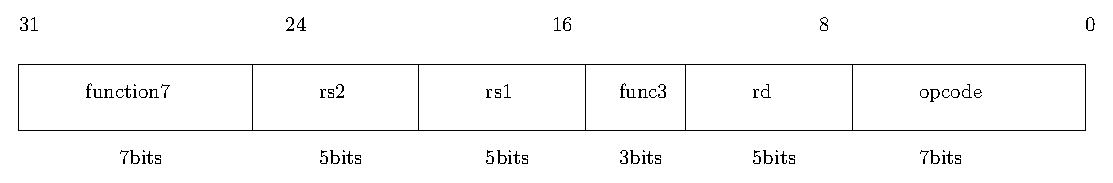
\includegraphics[width=10cm,height=2cm]{images/riscv.eps}
\end{center}
includegraphics 裡面的設定除了width height,還有放大跟旋轉
\begin{itemize}
\item scale=1.5
\item angle=45
\end{itemize}

\subsection{基本表格}
表格也是很常使用的一種元素,基本表格用 tabular ,他的延伸使用
tabular*, 但有些寬度高度是用一些技巧例如用 \verb=\\[-1pt]=
多加行列的控制不是很直觀, 加上tabularx, array 兩個 package 可以控制更多
的寬度高度線條粗細。而 colortbl 則是有簡單設定顏色的 package。
\begin{verbatim}
\begin{tabular}[b]{|p{3cm}@{\Large 大文字}rr||c}
r1c1 & r1c2 & r1c3 \\
\hline
\hline
r2c1 is a very long paragraph 
that we can have new line automatically 
with \verb=p{}= & r2c2 & r2c3 becomes longer & r2c4 becomes longer  \\
     & r3c2 & r3c3 & small \\
r4c1 & r4c2 & r4c3 & a \\
\cline{2-3}
\multicolumn{2}{|c}{r5c1} & r5c2 & r5c3 \\
\hline
\end{tabular}
\end{verbatim}
表現效果
\begin{center}
\begin{tabular}[b]{|p{3cm}@{\Large 大文字}rr||c}
r1c1 & r1c2 & r1c3 \\
\hline
\hline
r2c1 is a very long paragraph 
that we can have new line automatically 
with \verb=p{}= & r2c2 & r2c3 becomes longer & r2c4 becomes longer  \\
     & r3c2 & r3c3 & small \\
r4c1 & r4c2 & r4c3 & a \\
\cline{2-3}
\multicolumn{2}{|c}{r5c1} & r5c2 & r5c3 \\
\hline
\end{tabular}
\end{center}
總之
\begin{itemize}
\item 畫整條橫線用 \verb=\hline= 合併欄位畫部份用 \verb=\cline{}=。
\item 畫直線 必須在一開始 tabular 環境設定。合併欄位時會自動不畫。
\item 新row 用換行 \verb=\\=
\item 新column \verb=&=
\item 合併 在 multicolumn 設定。
\item 對齊 必須在 tabular 環境一開始設定,跨欄對齊在 multicolumn 設定。
\end{itemize}
其中\\
\verb=[]=是整個 table 與外面本文文字對齊上中下選項
\begin{itemize}
\item t, c, b 表示整張 table 與外面本文文字對齊 top, center, bottom。
\end{itemize}
\verb={}= 表示格子裡面文字欄位選項
\begin{itemize}
\item l, c, r 表示欄位內文字對齊 left, center, right,並沒有高低對齊。
\item | 表示畫直線
\item \verb=p{width}= 指定欄位真正寬度,p 是 paragraph,
用 p 的功能來讓文字多時能自動換行, 在 tablular 裡面要用 verbatim, 
listings 要用這個。 這無法再指定文字對齊,
內定是對齊 top,但加上 array package 可以多上 m 與 b,
一個是對齊 middle ,一個是對齊 bottom。
\item \verb=@{font macro}= 指定整欄位文字效果。
這也無法再指定文字對齊與寬度,就是多一欄,然後
上面的 lcr 跟 p 都跟這欄位沒有關係,它跟隔壁欄位間距設為0。
\item tabular 如果沒有用 p ,則是不會自動折行的,會一直跑出欄位,
因此最後一欄通常要使用 p 功能,來讓文字停在一定範圍內。或者用
tabularx 其他更好功能。
\end{itemize}
合併欄位
\begin{itemize}
\item \verb=\cline{2-3}= 指定劃直線只畫到何處 2--3 就是畫 2--3 兩欄。
只有跨 column 沒有跨 row ,因為跨 row 其實是兩行 row 中某 row 欄位是空,
然後不劃線而已。
\item \verb=\multicolumn{count}{l|c|r}{xxx}= 從這個欄位跨 count 並且把文字 xxx 靠
l c r 對齊,第二個 \verb={}= 跟上面的意思一樣的。
\end{itemize}
用 tabular 是可以巢狀下去的,一個 tabular 裡面可以再另一個
,所以在對齊上面是很有用的。

\subsection{浮動處理與文繞圖表}
浮動 floating 是專業排版中的大圖表與圖表列表整理的重要處理,除了自動計算
大圖表的距離空白等美觀與置放點外, 都會提供一個
caption 選項,會自動幫你計算圖表數量,在書籍前後可以列出來參考。
\\\\
而文繞圖表很多在雜誌編排上會出現。

\subsubsection{浮動處理}
floating 的用法是要用
\begin{itemize}
\item \begin{verbatim}
\begin{figure}
  \caption{xx}\label{fig:myfig}
  \includegraphics{...}
\end{figure}
\end{verbatim}
\item \begin{verbatim}
\begin{table}
  \caption{xx}\label{tab:mytab}
  \begin{tabular}
    ...
  \end{tabular}
\end{table}
\end{verbatim}
\end{itemize}
\begin{figure}
\caption{浮動圖形範例}
\centering
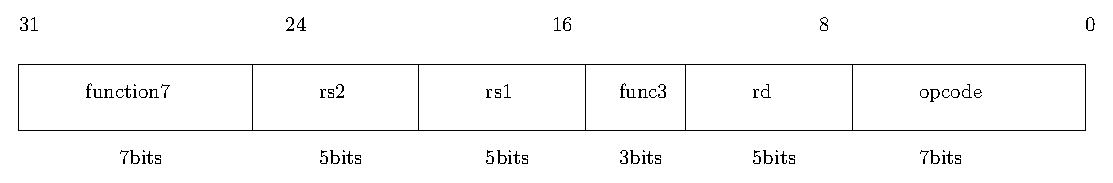
\includegraphics[width=5cm,height=2cm]{images/riscv.eps}
\end{figure}

\begin{table}
\centering
\caption{浮動表格範例}
\begin{tabular}{ccc}
a & b & c \\
\hline
1 & 2 & 3
\end{tabular}
\end{table}
table 的選項強制不要浮動選項,here 的選項,
\begin{itemize}
\item \verb=\begin{figure}[h]=
\item \verb=\begin{table}[h]=
\end{itemize}
或者單獨佔一頁 用 p 不用 h,p 通常會放在下一頁整頁。
\\\\
例如我用上
\begin{verbatim}
\begin{figure}
\caption{浮動圖形範例}
\centering
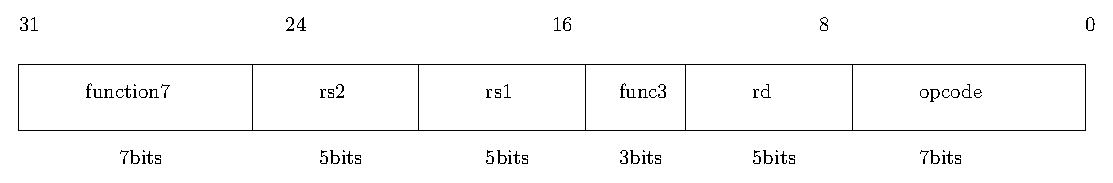
\includegraphics[width=5cm,height=2cm]{images/riscv.eps}
\end{figure}

\begin{table}
\centering
\caption{浮動表格範例}
\begin{tabular}{ccc}
a & b & c \\
\hline
1 & 2 & 3
\end{tabular}
\end{table}
\end{verbatim}
即使我沒有額外給\verb=\label=,它還是自動幫我做了 cross reference。
Table 跟 Figure。這可以自己在table figure 環境裡面設定 label
讓自己在文章中用 ref pageref 來參照。只是 label 必須在 caption
之後使用。

\subsubsection{文繞圖表}
如果圖表是小小的只佔頁面寬度的某部份, 本文文字跟
圖表大 object 看空間還夠不夠,放得下就放,這時圖表只是一個很大的字而已。
這時要對齊就要用 tabuler 中的 tcb 對齊上中下選項。內定 tabular 是 center,
 而 includegraphics 一律對齊 bottom 。這時並沒有 text-wrapping。
\\\\
例如這是小 table 
\begin{tabular}{cc}
title & item \\
\hline\hline
a & b
\end{tabular}
與後面文字。
\\\\
這是小圖 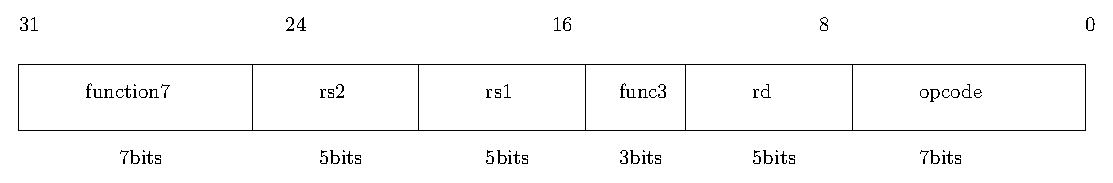
\includegraphics[width=5cm,height=5cm]{images/riscv.eps} 跟它後面的文字。
\\\\
而之前用 includegraphics 與 tabular 時,我為了好看都已經用上
 \verb=\begin{center}=了,所以用 center 環境會佔滿整個頁面做 object,因此
也就看不到文字與圖表並列排版與文繞圖表了。此時像 tabular 的可選擇參數的
 t,c,b 是沒有意義的。而 使用 table, figure floating 時,由於會有
 caption ,所以 caption 都是整頁中間文字,因此也沒有文字圖表這種對齊問題。
\\\\
如果想要圖表邊的空白也填滿文字,那就要文繞圖表,要用 
\href{https://mirror.math.princeton.edu/pub/CTAN/macros/latex/contrib/wrapfig/wrapfig-doc.pdf}{wrapfig} package
例如繞表格用 wraptable
\begin{verbatim}
\begin{wraptable}{r}{0pt}
  \begin{tabular}{cc}
  title & effect \\
  \hline\hline
  a & b \\
  \hline
  c & d \\
  \hline
  e & f 
  \end{tabular}
\end{wraptable}
\end{verbatim}

\noindent
試著寫一大段文字,在圖表旁邊看會長怎樣,如果長的醜,就不要用了,如果長的漂亮,還
值得學習這個 package ,不然就是浪費時間學習,閱讀,測試。

\begin{wraptable}{r}{0pt}
%\centering
  \begin{tabular}{cc}
  title & effect \\
  \hline\hline
  a & b \\
  \hline
  c & d \\
  \hline
  e & f 
  \end{tabular}
  %\caption{\label{wraptable}文繞圖表格}
\end{wraptable}

\noindent
合格者には日本語能力認定書を送ります。また、日本国内での受験者全員に合否結果通知書を送ります。
海外での受験者には2014年から合否結果通知書のかわりに証明書を全員に送ります。
日本国内の場合、第1回(7月)試験の結果は9月上旬、第2回(12月)試験の結果は2月上旬に送る予定です。
海外の場合は、受験地の試験実施機関を通じて送りますので、
第1回(7月)試験の結果は10月上旬、第2回(12月)試験の結果は3月上旬に受験者に届く予定です

\noindent
繞圖形要用 wrapfigure
\begin{verbatim}
\begin{wrapfigure}[4]{l}{0.5\textwidth}
\centering
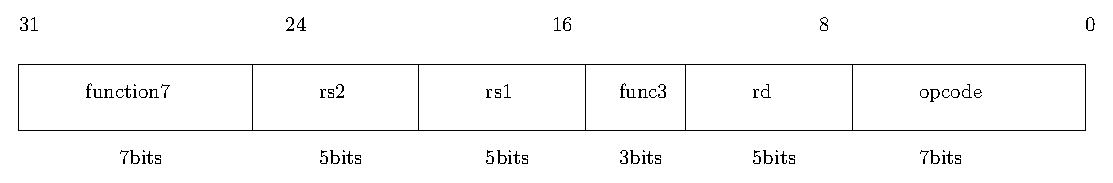
\includegraphics[width=0.48\textwidth]{images/riscv.eps}
\end{wrapfigure}
\end{verbatim}

\noindent
試著寫一大段文字,在圖表旁邊看會長怎樣,如果長的醜,就不要用了,如果長的漂亮,還
值得學習這個 package ,不然就是浪費時間學習,閱讀,測試。

\begin{wrapfigure}[4]{l}{0.5\textwidth}
  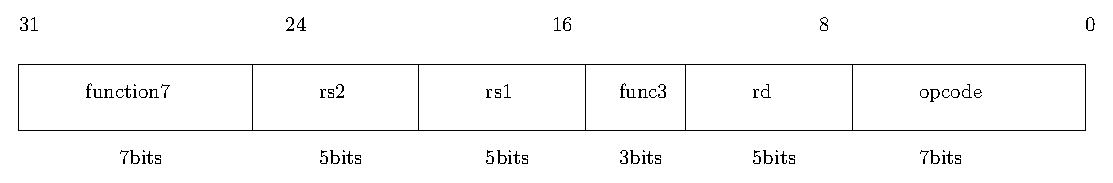
\includegraphics[width=0.48\textwidth]{images/riscv.eps}
  %\caption{\label{riscv}RISC-V Insturction Set format}
\end{wrapfigure}

合格者には日本語能力認定書を送ります。また、日本国内での受験者全員に合否結果通知書を送ります。
海外での受験者には2014年から合否結果通知書のかわりに証明書を全員に送ります。
日本国内の場合、第1回(7月)試験の結果は9月上旬、第2回(12月)試験の結果は2月上旬に送る予定です。
海外の場合は、受験地の試験実施機関を通じて送りますので、
第1回(7月)試験の結果は10月上旬、第2回(12月)試験の結果は3月上旬に受験者に届く予定です
\\\\
選項
\begin{itemize}
\item 第一個非必要選項是繞圖表文字是幾行。
\item r, R, l, L,  位置選項,圖表在文字右邊左邊,大寫表示 float ,小寫表示就在原地。
所以通常用小寫。
\item 圖表寬度。所以應該都是跟 includegraphics 或 tabular 的 p 設定差不多大小。但
wrap 的大小要稍微大一點,不然也可設 0pt。
\end{itemize}
測試的結果有點不如想的準確,或許它會自動計算,還有 wrapfigure wraptable 前後
要有字,也要空白一行,也就是必須是獨立的 paragraph 才會動作,也有看到有說第
一個選項也要設定不然不會動或者走鐘去。

\section{排版注意事項}
有些排版特有的觀念與注意事項是我們之前一直在提醒的,另外還有的是 {\LaTeX} 處理
時的一些特別行為。
\subsection{出版商的專業術語}
\begin{itemize}
\item break line 強迫斷行使用 \verb=\\ 或 \newline=, \verb=\\[2cm]=
表示斷行後加個空白行兩公分。然後 每次的斷行不管自動或強迫的都會在兩行間補一個
空白。 但不是那麼剛好每個字的寬度排
起來後可以填滿一行,因此在每行最後有可能英文字會被拆成兩半,
這也是有規矩的,英文不像中文是方塊字,而是會用 hyphen rule 把一個 word 拆兩半。
\item space 空白,除了在換行時會加空白,在句子與句子中間,應該要多一點空白,這
是排版軟體看到標點符號 \verb= . ? :=, %stopzone
自動幫我們做的。但有時一些縮寫像 \verb=etc. i.e Mr.=,這種就要強迫它不特別空白,
可以用 \verb=~=, 或者\verb=\ =,兩種都可以表示正常空白。而不同字體間的空白大小
其實也都有嚴格規定只是排版軟體幫我們做掉而已。
\item indent 縮排是預設每個章節的第一個段落的第一行是不縮排,
從第二個段落開始才會內縮。所謂的段落除了用\verb=\paragraph{}= 外,在文字編輯
器上多加一個空白行就是新段落,因此比寫程式還嚴格。如果不要縮排就在空白行前
加上 \verb=\noindent=。
\item 引號 跟 shell 一樣,backquote, single quote, double quote 用法在排版界
是有不同詮釋的,所有的引號都是需要有左右夾起來的。
\begin{itemize}
\item single quote 單引號必須用真的 backquote + 1 個真的 single quote。
\item double quote 雙引號反而必須用兩個真的 backquote + 兩個真的 single quote
\end{itemize}
也就是原本鍵盤上的 backquote 變成左邊倒勾的引號符號,鍵盤上 single quote 
變成右邊正勾的符號。 如果真想用原本的電腦上看到的樣子,只能用verbatim。
使用 \verb=\verb 或者 begin{verbatim}= 也有效。\\\\
`倒引號`, `排版單引號', '錯誤單引號', ``排版雙引號'', "錯誤雙引號"\\\\
用 verbatim 原型變成\\\\
\verb= `倒引號`=, \verb='單引號'=, \verb=``排版雙引號''=, \verb="雙引號"=\\\\
\item 三點 \dots 要用 \verb=\dots 或者 \ldots= ,不要直接用鍵盤的 ... 。
\item 破折號與減號在英文排版上。 正式有分 hyphen, en-dash, em-dash 三種。
hyphen 長度最短,en-dash 大概
是 N 這個字長度, em-dash 是 M 這個字長度。hyphen 用來表示一個單一字彼此有關係
例如 son-in-law 或者在斷行時表示前後字元是一個字。en-dash 表示一段範圍,例如
 1 -- 10, em-dash 表示句子的分開額外的意義說明,例如花好香 --- 帶有淡淡的牛奶香。
  \begin{itemize}
    \item Hyphen: 使用 \verb=-=
    \item En-dash: 使用 \verb=--=或者\verb= \textendash=
    \item Em-dash: 使用  \verb=---=或者 \verb=\textemdash=
  \end{itemize}
負號則須用數學的\verb=$-$=。
\end{itemize}
另外有引言的 quote 表現用 \verb=\begin{quote} ... \end{quote}=
\begin{quote}
引言,子曰三日不讀書,言語無味面目可憎。
\end{quote}
總之輸入的換行 newline,空白 space,空白行 empty line,轉成排版時有特殊轉換,
而輸入的多個連續空白就只有一個空白,多個連續空白行就只有一個空白行,
還有鍵盤上的符號在正規嚴謹的排版要求下,是會長成不同樣子的,因此要看你要求
嚴不嚴格,用排版軟體的特殊命令,用脫逃字元,用 verbatim,與單用鍵盤打出字元
長相到最後排版都會不同,所以要求一致性長相時,要注意使用。

\subsection{latex 注意事項}
\begin{itemize}
\item table of content 要跑兩次引擎,第一次跑出 .toc 檔,才能產出漂亮的 TOC。
      cross reference label ref 也要。
\item index 產生還要在兩次中間跑 makeindex 程式。
\item 命令是從反斜線後第一個字母開始,到第一個非字母符號為止(包括空
白、標點符號及數字)。因此:\verb={\LaTeX}= 與 \verb=\LaTeX{}= 與 
\verb=\LaTeX = ,作用正常講會不一樣,也就是 \verb=\comand= 與\verb=\command   =
正常講是兩個不同命令。只是後面 macro 程式幫你作掉變一樣而已。排版時要小心
尤其是 logo 形式的命令,還是要用\verb={\logo}=形式,不然會 logo 跟字間沒有
空白。
\item 註解符號(\%),可以放在一行的任何地方,\% 後的文字會被 {\LaTeX} 忽略。
所以,如果是放在一行的最尾端,那麼 {\LaTeX} 會自動插入的斷行空白也將會被忽略,
另外在 vim 中的語法顏色有的會出錯,也是用 \%stopzone 想辦法把它改回來。
\item \verb=\\= 斷行要小心,paragraph, end 環境等後面不能直接跟著它,會出錯。
\end{itemize}

\subsection{中文注意事項}
\begin{itemize}
\item 使用 \% 在尾巴消除一些自動英文空白。以前如果沒有加,就會每個中文字斷行地方
看起來多一個空白,怪怪的。新的 xeCJK package 做的好一點。
所以已經不需要像以前在屁股尾巴加上 \%,但這還是在很多地方很好用的技巧。
\item 斷行,空白,符號的使用規矩跟英文的會有點不一樣。但這也要看期刊,
單位的要求為何,或許有 {\LaTeX} 的特殊版本使用。
\end{itemize}

\subsection{其他}
vim 中打開 :syntax on,開 tex 檔會自動有基本語法顏色,可是用上特別的
 package 後,會走鐘掉。最基本的修正就是在亂掉地方加上註解 
\verb=%stopzone=。 但 package 太複雜跟其他的 macro 有衝突。例如 lstlistings
的 vim 的配合,用 \verb=%stopzone= 與多加一個檔案
\verb=$HOME/.vim/after/syntax/tex/lstlistings.vim=
\begin{footnotesize}
\begin{verbatim}
syn region texZone start="\\begin{lstlisting}" end="\\end{lstlisting}\|%stopzone\>"
syn region texZone  start="\\lstinputlisting" end="{\s*[a-zA-Z/.0-9_^]\+\s*}"
syn match texInputFile "\\lstinline\s*\(\[.*\]\)\={.\{-}}" contains=texStatement,texInputCurlies,texInputFileOpt
\end{verbatim}
\end{footnotesize}
\clearpage
